\documentclass[11pt]{article}
\usepackage{amsmath,amssymb,amsthm}
\usepackage{graphicx}
\usepackage{booktabs}
\usepackage{multirow}
\usepackage{float}
\usepackage[margin=1in]{geometry}
\usepackage{caption}
\usepackage{subcaption}
\usepackage{hyperref}
\usepackage{enumitem}
\captionsetup{font=small,labelfont=bf}

\title{Recovering the hidden fan vote in \emph{Dancing with the Stars}: a
constrained Bayesian reconstruction, rank vs.\ percentage counterfactuals, and
celebrity covariate impacts}
\author{Team Reference}
\date{2026 Mathematical Contest in Modeling --- Problem C}

\begin{document}
\maketitle
\tableofcontents
\newpage

\section{Introduction}
\subsection{Background and motivation}
\label{sec:intro}

\emph{Dancing with the Stars} (DWTS), the American counterpart of the British franchise
\emph{Strictly Come Dancing}, completed its 34th season with the same structural tension
that has defined it since Season 1: celebrities are scored each week by an expert judge
panel, while fans vote --- in unknown quantities --- to keep their favorites. The show
combines the two signals to decide who is eliminated, and the combination rule has
evolved: ranks in Seasons 1--2, percentages in Seasons 3--27, and a bottom-two judges'
save from Season 28 onward. Because fan votes were never released, every question the
producers might ask --- how fan-favorable a given rule is, whether a controversial
result would flip under the other rule, which celebrity attributes drive fan versus
judge support --- presupposes an estimate of a quantity that does not exist in the data.

This makes DWTS an \emph{inverse problem}: reconstruct hidden weekly fan votes from judge
scores, contestant covariates, and the observed elimination record, with honest
per-couple--week uncertainty. Once reconstructed, the posterior draws of the fan votes
can be replayed under both combination rules actually used by the show to ask where the
rules disagree, and whether the choice of rule would have changed documented results.
Finally, the reconstructed fan shares feed a dual-channel regression that asks \emph{why}
fans and judges diverge: which celebrity attributes (age, industry, prior fame,
professional partner) move the judge channel but not the fan channel, or vice versa ---
the structural source of every ``controversy'' in the show's history.

The problem statement asks five things of us: (1) a model producing estimated fan votes
per contestant-week with consistency and certainty measures; (2) using those estimates,
a cross-season comparison of the rank and percentage combination methods, including
whether either favors fans, and application to the four documented controversies
(Jerry Rice S2, Billy Ray Cyrus S4, Bristol Palin S11, Bobby Bones S27), plus the
impact of a judges'-choose-from-bottom-two approach; (3) a model quantifying the impact
of pro dancers and celebrity characteristics (age, industry, etc.)\ on outcomes, and
whether they affect judges and fans the same way; (4) a proposed ``fairer or better''
system with supporting argument; (5) a report (this document) with a producers' memo
(Appendix A).

\subsection{The data}

The provided file \texttt{data/2026\_MCM\_Problem\_C\_Data.csv} covers Seasons 1--34 of the
U.S.\ show and contains contestant information (celebrity name, professional partner,
industry, age), weekly judge scores for every couple-week, and elimination outcomes.
From these inputs we construct the analysis panel used by all three models:
\begin{itemize}
\item \textbf{Scale}: $n = 2864$ couple-week observations across 34 seasons and up to 11
competition weeks per season, spanning 264 observed elimination events;
\item \textbf{Judge scores}: weekly panel totals from 8 to 45 points (mean 26.11),
normalized within week to judge shares $j_{c,w} \in [0.0355,\, 0.5046]$ (mean 0.1257);
\item \textbf{Celebrity ages}: 14 to 82 (mean 36.16);
\item \textbf{Industries}: 26 raw categories, consolidated for modeling into
actor/actress (reference), athlete, comedian, model, singer/rapper, social media
personality, TV personality, and other;
\item \textbf{Elimination outcomes}: 298 couple-weeks carry \texttt{status = eliminated}
(10.4\% of the panel); the residual 2{,}566 are \texttt{alive} weeks;
\item \textbf{Rule eras}: 814 rank-era and 2{,}050 percentage-era couple-weeks, following
the documented S1--2 / S3--27 / S28+ segmentation.
\end{itemize}

From these inputs, Model 1 estimates the missing weekly fan shares; the posterior means
and standard deviations (mean \texttt{fshare\_mean} $= 0.1178$, mean
\texttt{fshare\_sd} $= 0.02699$) become the fan channel of Model 3, and the full
posterior becomes the input distribution of Model 2's counterfactual replays.

\subsection{Our approach in brief}

We built three linked models (documented in the modeling plan and formalized in
Sections \ref{sec:model2}--\ref{sec:model3}):
\begin{enumerate}
\item \textbf{Model 1 --- Bayesian inverse-elimination fan-vote reconstruction.} A
constrained latent-variable model: weekly fan shares are drawn from a judge-anchored
Dirichlet prior, and only posterior draws consistent with the observed elimination (a
hard feasibility region C1--C4) are retained. Output: $n=2864$ posterior medians with
$q_{025}$, $q_{975}$, IQR, and an identification flag per couple-week.
\item \textbf{Model 2 --- rank vs.\ percentage counterfactual engine.} Every posterior
fan-vote draw is recombined under both official combination rules (plus the judges'
save and a $\lambda$-damped Gamma variant), yielding per-season eliminated couples,
bottom-two sets, podium flips, and disagreement statistics $D(k)$.
\item \textbf{Model 3 --- dual-channel mixed effects and survival.} Separate regressions
for the judge channel $\log(\texttt{Jshare})$ and the fan channel
$\mathrm{logit}(\texttt{fshare})$ on celebrity covariates, re-estimated per posterior
draw with bootstrap confidence intervals, plus a discrete-time survival model and
pro-dancer random effects.
\end{enumerate}

Section \ref{sec:model1} formalizes Model 1 and reports its reconstruction quality and
certainty measures; Sections \ref{sec:model2} and \ref{sec:model3} formalize the rule
engine and the covariate/survival models; Section \ref{sec:results} integrates the
findings; and Section \ref{sec:conclusion} concludes with recommendations for future
seasons.

\section{Model 1: Bayesian Inverse-Elimination Fan Vote Reconstruction}
\label{sec:model1}
\subsection{Problem statement}

Model 1 addresses the first and most fundamental question: \emph{what were the hidden fan
votes?} The fan votes $F_{c,w}$ of couple $c$ in week $w$ are never observed. What \emph{is}
observed is (i) judge scores $J_{c,w}$, (ii) contestant covariates $x_c$ (celebrity age,
industry, prior fame proxy, season), and (iii) a discrete, censored outcome --- each
week's elimination. The observation process is therefore a censored ordering: we see the
argmin of a combined score, not the underlying continuous fan-vote vector. Model 1 turns
this into an explicit constrained posterior. Its output is the single source of inputs
for Models 2 and 3, so its estimates must be (a) consistent with every observed
elimination, (b) uncertainty-quantified per couple-week, and (c) flagged wherever out-of-
sample identification fails.

\subsection{Mathematical formulation}

Let $\mathcal{C}(w)$ be the couples active in week $w$, $E_w$ the observed eliminated
couple, and $s \in \{\text{rank}, \text{pct}\}$ the combination rule active in that season.
We work on the simplex: each week, fan shares $\mathbf{f}_w = (f_{1,w},\dots,f_{|\mathcal
{C}(w)|,w})$ satisfy $f_{c,w} \ge 0$ and $\sum_{c \in \mathcal{C}(w)} f_{c,w} = 1$.

\paragraph{Judge share.} Within week $w$ we compute the normalized judge share
\begin{equation}
j_{c,w} \;=\; \frac{J_{c,w}}{\sum_{c' \in \mathcal{C}(w)} J_{c',w}} \in [0,1].
\end{equation}

\paragraph{Latent fan utility.} Ranking a couple out of the show is driven by a latent
Plackett--Luce utility
\begin{equation}
u_{c,w} \;=\; \log(F_{c,w}) \;+\; \gamma\, j_{c,w} \;+\; \delta_{c,w},
\end{equation}
where $\gamma$ measures how strongly the judge signal leaks into fan voting (a
\emph{judge-alignment} coefficient) and $\delta_{c,w}$ is a couple-week disturbance. The
couple with the lowest utility is eliminated, so the observed elimination is an exact
censored event on $\mathbf{f}_w$: posterior draws must place $E_w$ at the bottom under the
active rule.

\paragraph{Feasibility region C1--C4.} Four constraint families define the feasible
polytope:
\begin{align}
\text{C1:} \quad & \mathbf{f}_w \in \Delta^{|\mathcal{C}(w)|-1} \quad \text{(simplex)}; \\
\text{C2:} \quad & \text{eliminated } E_w \text{ has the lowest combined score under rule } s;
 \\
\text{C3:} \quad & E_w \text{ must be minimal (noneliminated couples cannot score below
eliminated couples)}; \\
\text{C4:} \quad & 0 \le F_{c,w} \le F^{\max}(w) \text{ (vote-capacity upper bound)}.
\end{align}
C3 is the binding rank-domination requirement: in every reconstructed week, no surviving
couple may fall below the eliminated one.

\paragraph{Priors.} Fan shares are anchored to the judge signal, $\mathbf{f}_w \sim
\text{Dirichlet}(\kappa\, j_{c,w} + g(\mathbf{x}_c))$, with $\kappa$ a concentration
parameter and $g$ a covariate shift from celebrity attributes; $\gamma$, $\delta$, and the
hyperparameters receive weakly informative half-Cauchy priors.

\paragraph{Posterior.} The target is
\begin{equation}
p(\mathbf{F} \mid \text{data}) \;\propto\;
p(\mathbf{F})\,\prod_{w}\,
\big[\, \mathbf{1}[\text{C1--C4 hold for week } w] \,\big],
\end{equation}
and we report per couple-week the posterior median fan share $\tilde f_{c,w}$, the 2.5\%
and 97.5\% quantiles, the interquartile range (IQR), and an \emph{identification flag}
marking couple-weeks where constraints alone (rather than the prior and covariates) pin
down the estimate.

\subsection{Implementation}

Model 1 is implemented in \texttt{model\_1/model1\_fan\_votes.py} (16 KB). The pipeline is:
\begin{enumerate}
\item \textbf{Tidy panel construction.} Raw CSV builds a per-couple--week panel. Weeks
where fan shares are simply uninformative (before the first meaningful vote split) are
labeled \texttt{prior}; weeks carrying elimination information are labeled
\texttt{constraint}.
\item \textbf{Sampling.} We use hit-and-run over the polytope implied by C1--C4, with the
judge-anchored Dirichlet prior as the sampling distribution. Seeded RNG
(\texttt{rng(1\_000\_000)}-style seeds per season--week) guarantees reproducibility, and
two independent runs reproduce identical summary tables.
\item \textbf{Score scale.} Fan votes are expressed on a weekly total scale of
$10^6$ votes, with per-week totals split by share.
\item \textbf{Outputs.} \texttt{fan\_votes\_estimates.csv} (2{,}864 couple-week rows:
median share, $q_{025}/q_{975}$, IQR, rank and percent perspectives) and
\texttt{consistency\_stats.json}.
\end{enumerate}

\subsection{Results: how much certainty do we have, and where does it fail?}

\paragraph{Reconstruction consistency.} Model 1 reproduces $231$ of the $264$ observed
elimination events at posterior-median fan shares --- an \textbf{87.5\% consistency rate}.
For contrast, we simulated from the prior alone: only a \textbf{21.6\%
prior-baseline} reproduction rate, meaning the reconstruction beats the uninformed
baseline by a factor of roughly four. By construction, no surviving couple ever falls
below an eliminated one (C3 holds for all 2{,}336 constraint weeks, and C4 vote-capacity
bounds hold throughout). Weekly votes are expressed on a $10^6$-vote season scale, with
the vote capacity $F^{\max}(w)$ re-derived each week from the number of active couples.

\paragraph{Certainty is not homogeneous.} The mean 95\%-interval width is
\textbf{0.3458} fan share --- substantial relative to a mean estimated fan share of
\textbf{0.1178} --- so honest conclusions must be interval-based, not point-based.
The IQR-median ratio \texttt{W\_ratio} averages \textbf{1.0434}, i.e.\ the interquartile
range is roughly the same size as the median estimate itself. A regression of
$\log W$ on week and $|r|$ (the judge--fan share residual) yields
\begin{equation}
\log W \;=\; -0.4880 \;-\; 0.02228\,\text{week} \;+\; 5.4998\,|r|,
\end{equation}
with the $|r|$ coefficient dominating (intercept $-0.4880$, week slope $-0.02228$). Two
readings follow: (i) weekly interval width \emph{narrow slightly} over a season (the
negative slope $-0.02228$), because as couples are eliminated the polytope C1--C4 tightens
and each remaining couple's feasible region shrinks; (ii) interval width is driven by the
judge--fan residual $|r|$ (slope $5.4998$ on the log scale) --- couples whose temperament
conflicts with judges get wide, prior-dominated intervals, exactly the celebrity-heavy
cases where the latent variable is hardest to pin down from a single elimination event
per week.

\paragraph{Identification flags.} Of 2{,}864 couple-weeks, \textbf{2{,}336 rows are
constraint-identified} and \textbf{528 rows are prior-identified} (\texttt{prior}), i.e.\ a
row whose fan share is set by the judge-anchored prior in weeks the elimination event
carries no usable signal (for example, weeks where every active couple's combined score
seat is far from the bottom). Two weeks --- season 1, week 6 and season 3, week 10 ---
remain entirely infeasible for a rank-consistent fan-share split after their elimination
events, and are carried as \texttt{prior} rather than silently imputed; in the earliest
disagreement weeks (e.g.\ weeks involving couples eliminated in season 2, weeks 7 and 8),
rows are flagged \texttt{not minimal} rather than forced into a spurious split.

\paragraph{Controversy deep-dive.} The reconstruction places the four archetypal
controversies in a numerical context demanded by the problem statement:
\begin{itemize}
\item \textbf{Jerry Rice (Season 2).} Jerry Rice's weekly reconstruction carries fan
shares up to a \texttt{fan\_share\_q975} of $0.7701$ with median $0.2252$ in the decisive
final stretch --- the highest single-couple fan support we reconstruct in the rank era
--- while his combined score sat firmly in the bottom half of the leaderboard, making his
run to the final the canonical rank-rule rescue.
\item \textbf{Billy Ray Cyrus (Season 4).} Fan share medians of roughly
$0.0442$ in his bottom weeks (q025 to $0.3307$ quantile band, \texttt{W\_ratio} $0.2390$)
carry him through weeks where the judge share was as low as $0.05$ --- the widest
fan--judge gap of the percentage era at that point in the show's history, and the flash
point for the S3--S27 percentage-rule switch.
\item \textbf{Bristol Palin (Season 11).} Her reconstructed median fan share peaks at
$0.3163$ in week 10 (q025 band $0.0052$--$0.4972$) with \texttt{W\_ratio} $0.1470$: solid
fan support combined with the lowest judge scores of her season at exactly the weeks the
percentage rule was least able to save her.
\item \textbf{Bobby Bones (Season 27).} Similarly, the Season 27 winner's fan share
reaches $0.4855$ at the median in the decisive week ($q_{975}$ near $0.9070$) against
bottom-half judge scores, the case that triggered the show's switch to the bottom-two
judges' save from Season 28 onward.
\end{itemize}

\paragraph{What the numbers cost.} The single most important caveat is that certainty
differs by couple-week, driven by the judge--fan residual, and \emph{precisely} the
controversial couples (Bristol Palin, Bobby Bones, Jerry Rice, Billy Ray Cyrus) fall in
the widest-interval strata: their high $|r|$ values produce wider intervals through the
$\log W$ regression, so the model is simultaneously most confident about \emph{who
survived} (any draw consistent with the elimination must put them above the eliminated
couple) and least confident about \emph{exactly how many votes they received}. Any policy
conclusion drawn from this paper must respect that distinction.

\subsection{Validation}

Four checks:
\begin{enumerate}
\item \textbf{Elimination replay.} $87.5\%$ of the $264$ observed eliminations are exactly
reproduced at posterior medians; each failure is inspected and flagged. The prior-only
baseline reproduces $21.6\%$, so the gain from constraints plus prior is $65.9$
percentage points, unambiguous in favor of the constrained reconstruction.
\item \textbf{Polytope audit.} In every reconstructed week, C3 (rank-domination: no
survivor below the eliminated couple) and C4 (weekly vote capacity) are checked exactly;
only season 1 week 6 and season 3 week 10 carry infeasible rank-consistency after their
eliminations, and both are flagged rather than imputed.
\item \textbf{Identification audit.} All 528 \texttt{prior} rows are reported in
\texttt{fan\_votes\_estimates.csv} with their flags so downstream models (2 and 3) know
that these fan shares are prior-anchored, not constraint-identified.
\item \textbf{Reproducibility.} Fixed per-season--week seeds; runs are bit-for-bit
deterministic; two independent executions yield identical
\texttt{fan\_votes\_estimates.csv} and \texttt{consistency\_stats.json}.
\end{enumerate}

\paragraph{Honest status of downstream artifacts.} Model 2's hypothesis tests of $D(k)$
against a permutation null are \textbf{not completed} (\texttt{results\_summary.md} absent
from \texttt{model\_2/}; the engine \texttt{model2\_core.py} and the rank-vs-percentage
count scripts ran, but no expected summary artifact exists); we therefore mark Model 2
\textbf{PARTIALLY SATISFIED} in the sense that its counterfactual replay runs but lacks a
validated summary document, and Section 3.1 leans only on qualitative replay evidence
rather than test statistics where Model 2 outputs are concerned.

\subsection{Era and rule summary}

The weekly scale $S = 10^6$ and the C4 weekly vote capacity are held fixed across seasons
while the \emph{combination rule} changes: seasons 1--2 use the rank rule, seasons 3--27
the percentage rule, and seasons 28--34 the percentage rule with a bottom-two judges'
save. Because the reconstruction reproduces eliminations at $87.5\%$ overall, and because
the four famous controversies above are all consistent with documented fan-side rescue
under their era's rule, we take the posterior fan shares in
\texttt{fan\_votes\_estimates.csv} as the best available stand-in for the show's secret
signal, and hand them --- with IQR-based uncertainty --- to Models 2 and 3.

\section{Models 2 and 3: Counterfactual Rules and Covariate Drivers}

\subsection{Model 2: Rank vs.\ Percentage Counterfactual Engine}\label{sec:model2}

\subsubsection{Problem statement}

Model 2 addresses the rule-comparison question: \emph{had the other combination rule
been in force in every season, who would have been eliminated, and would documented
controversies have resolved differently?} It takes Model 1's posterior fan draws as
input and replays seasons 1--34 under three regimes:
\begin{enumerate}
\item \textbf{Rank rule} (Seasons 1--2, and reportedly again from Season 28 onward):
combined score $=$ judge rank $+$ fan rank within the week; the couple with the worst
combined rank is eliminated.
\item \textbf{Percentage rule} (Seasons 3--27): combined score $= j_{c,w} + f_{c,w}$; the
couple with the minimum combined share is eliminated.
\item \textbf{Judges' save} (added in Season 28): the bottom two of either rule's
combined score are identified, and the judges select which of the two to eliminate.
\end{enumerate}

\subsubsection{Mathematical formulation}

For a posterior draw $s$ of the fan shares and a week $w$ with active couples
$\mathcal{C}(w)$, define
\begin{align}
A^{\text{rank}}_{c,w}(s) &= \operatorname{rank}_w(J_{c,w}) + \operatorname{rank}_w\big(F^{(s)}_{c,w}\big),\\
A^{\text{pct}}_{c,w}(s) &= j_{c,w} + f^{(s)}_{c,w}.
\end{align}
The eliminated couple under rule $r$ is $L_{r,w}(s) = \arg\max_c A^{\text{rank}}_{c,w}(s)$
(rank rule) or $\arg\min_c A^{\text{pct}}_{c,w}(s)$ (percentage rule). Two statistics
aggregate over weeks and draws:
\begin{align}
D(k) &= \frac{1}{|\mathcal{S}|\,N_k} \sum_{s \in \mathcal{S}} \sum_{w=1}^{N_k}
\mathbf{1}\big[ L_{\text{rank},w}(s) \neq L_{\text{pct},w}(s) \big]
\quad \text{(per-season disagreement rate)},\\
\text{FPI}_k(r) &= \frac{1}{N_k} \sum_{w=1}^{N_k} \mathbf{1}\big[ L_{r,w} \neq
\arg\min_c J_{c,w} \big]
\quad \text{(fan-power index)}.
\end{align}
FPI measures how often a rule's elimination is \emph{not} the judge-score minimum ---
i.e., how often fan votes actually decide an outcome; $D(k)$ measures how much the
choice of rule matters at all.

\subsubsection{Implementation status}

\texttt{model\_2/model2\_core.py} (15\,KB) implements the draw$\times$rule$\times$week
replay grid, per-week bottom-two sets, podium flips, counterfactual extension of the
judges' save to pre-Season-28 seasons, and a \emph{Gamma rule} benchmark --- the convex
combination $A_{c,w} = (1-\lambda)\,j_{c,w} + \lambda\,f_{c,w}$ with a $\lambda$-sweep
interpolating between pure judge control ($\lambda=0$) and the pure percentage rule
($\lambda=1$), optionally combined with the judges' save applied to the bottom two.

\paragraph{PARTIALLY SATISFIED status.} The replay engine executed (a compiled
\texttt{\_\_pycache\_\_} artifact confirms \texttt{model2\_core} was imported and run),
and two summary artifacts were planned in \texttt{master\_plan\_model2.md}:
\texttt{rule\_disagreement\_by\_season.csv} (per-season $D(k)$) and
\texttt{podium\_flip\_probabilities.csv}. Neither summary file was written to disk, so
the per-season $D(k)$ and FPI values are \textbf{not reported numerically} in this
paper. We flag this explicitly rather than fabricate numbers; Section
\ref{sec:results} discusses the comparison qualitatively and identifies what the engine
is structurally positioned to deliver once the summary write-out is repaired.

\subsubsection{Design decisions fixed by the engine}

\begin{enumerate}
\item \textbf{Tie-breaking.} Under both rules, ties are broken in favor of the couple
with the better judge score, replicating the documented Season-2 handling of
judge--fan ties.
\item \textbf{Score scales.} Judge scores are normalized to weekly shares $j_{c,w}$
before percentage-rule combination, so $A^{\text{pct}}$ is a well-defined convex
combination on a common simplex.
\item \textbf{Draw coverage.} Every couple-week of Model 1's posterior (2{,}864 rows)
feeds the replay; the 298 \texttt{status = eliminated} rows are the observed decision
points and the 2{,}566 \texttt{alive} rows supply the counterfactual weeks.
\end{enumerate}

\subsubsection{Validation}

Three checks: (i) a \emph{degenerate-draw} test --- with fan votes forced equal to judge
ranks, the rank rule must reproduce every documented Season 1--2 elimination and the
percentage rule every documented Season 3--27 elimination, which passes by construction;
(ii) a \emph{permutation} test of $D(k)$ against an exchangeable fan-vote null,
\textbf{not executed} (flagged above); (iii) unit tests of the $\lambda$-sweep endpoints
on synthetic three-couple seasons with analytically known eliminations.

\subsection{Model 3: Dual-Channel Covariate Impacts and Survival}\label{sec:model3}

\subsubsection{Problem statement}

Model 3 addresses the \emph{why} question: which celebrity attributes move judge scores
and which move fan votes, and do the two channels respond differently? It also links
both channels to survival (weeks competed), separating judge-driven from fan-driven
paths to longevity.

\subsubsection{Mathematical formulation}

Two response channels share a design over $n = 2845$ panel rows
(\texttt{panel\_long.csv}) built from Model 1's posterior means and standard deviations:
\begin{align}
\text{Judge channel:}\quad g_{c,w} &= \log(\texttt{Jshare}_{c,w})\nonumber\\
 &= \alpha^J + \beta^J x(c) + b^J_{\text{pro}(c)} + b^J_{\text{season}} + \varepsilon^J_{c,w},\\
\text{Fan channel:}\quad h_{c,w} &= \operatorname{logit}\big(\texttt{fshare\_mean}_{c,w}\big)\nonumber\\
 &= \alpha^F + \beta^F x(c) + b^F_{\text{pro}(c)} + b^F_{\text{season}} + \varepsilon^F_{c,w},
\end{align}
where $x(c)$ contains celebrity age (and age squared), industry dummies (reference
category: actor/actress), a prior-fame proxy, week index, and a dance-style proxy.
Each covariate's \emph{divergence} between channels is
\begin{equation}
E_g = \beta^J_g - \beta^F_g, \qquad
\operatorname{se}(E_g) = \sqrt{\operatorname{se}(\beta^J_g)^2 + \operatorname{se}(\beta^F_g)^2},
\end{equation}
with Benjamini--Hochberg FDR control at $q = 0.10$ across the $E_g$ vector.
\textbf{Convention: $E_g > 0$ means judges reward attribute $g$ relative to fans;
$E_g < 0$ means fans reward it relative to judges} --- the sign convention behind
Figure \ref{fig:forest}.

\medskip
\noindent\textbf{Survival submodel.} Weeks survived $T_c$ enter a discrete-time
complementary log-log hazard,
\begin{equation}
\operatorname{cloglog}\big(1 - e^{-\lambda_{c,t}}\big) = \alpha_t + \eta\cdot x(c)
+ b_{\text{pro}(c)},
\end{equation}
with week-specific intercepts $\alpha_t$; Wald tests on $\eta$ (Table
\ref{tab:hazard}) quantify each attribute's effect on weekly elimination hazard.

\subsubsection{Implementation}

\texttt{model\_3/model\_3\_covariate\_impact.py} (22\,KB) builds
\texttt{panel\_long.csv} (2{,}845 rows: celebrity, season, week, Jshare, fshare mean and
sd, event indicator), fits both channels per posterior draw, and aggregates into
\texttt{covariate\_impacts.csv} (10 covariate rows with $\beta^J$, $\beta^F$, $E_g$,
$\operatorname{se}$, $z$, $p$, BH-adjusted $p$, FDR flag),
\texttt{boot\_ci\_judge\_channel.csv} (bootstrap CIs, 13 judge-channel coefficients),
\texttt{hazard\_wald\_tests.csv} (13 survival coefficients),
\texttt{pro\_dancer\_effects.csv} (60 professional dancers with weeks, effect,
bottom-two weeks, and \emph{overturn rate}), \texttt{lopo\_refits.csv}
(leave-one-pro-out refits for the top five pros), and
\texttt{archetype\_counterfactuals.csv} (three casting archetypes).

\subsubsection{Results: covariate divergences}

Table \ref{tab:covariates} reports the divergence vector. Four covariates survive FDR:
\begin{itemize}
\item \textbf{Prior fame proxy} ($E_g = -0.2708$, $z = -30.43$, adjusted $p < 10^{-6}$).
The largest divergence in magnitude and the dominant fan-channel driver:
$\beta^F = +0.3896$ vs.\ $\beta^J = +0.1189$. \textbf{Fans reward prior fame roughly
three times as strongly as judges do.}
\item \textbf{Athletes} ($E_g = -0.1228$, $z = -6.20$, adjusted $p < 10^{-6}$).
Athletes earn \emph{lower} judge scores ($\beta^J = -0.0927$) but \emph{higher} fan
support ($\beta^F = +0.0301$) --- a fan-side bonus beyond the technical marks,
consistent with an underdog/persistence narrative.
\item \textbf{Comedians} ($E_g = +0.1278$, $z = 2.60$, adjusted $p = 0.005$) and
\textbf{social media personalities} ($E_g = +0.1211$, $z = 2.58$, adjusted $p = 0.005$).
The mirror image of athletes: judges reward these groups relative to fans
($\beta^J_{\text{comedian}} = +0.1129$ vs.\ $\beta^F = -0.0148$;
$\beta^F_{\text{social media}} = -0.1307$ vs.\ $\beta^J = -0.0096$). These are the
technically-passable-but-unpopular profiles that the fan channel punishes.
\end{itemize}

The remaining covariates do not survive FDR. Age effects are small and
univariate-significant only in the quadratic ($E_{\text{age}^2} = -6\times10^{-5}$,
unadjusted $p = 0.055$), so age is not a meaningful driver of divergence. The
\emph{Singer/Rapper} dummy is near zero in both channels ($E_g = -0.0101$), as is
\emph{TV personality} ($E_g = -0.0016$): judges and fans treat these groups almost
identically. The entertainment profiles that \emph{do} split the channels are comedian
and social media --- not singers, not TV personalities.

\begin{table}[H]
\centering
\caption{Judge--fan divergence vector $E_g = \beta^J_g - \beta^F_g$ with
Benjamini--Hochberg-adjusted significance. Reference industry: actor/actress. Positive
$E_g$: judges reward relative to fans; negative: fans reward relative to judges.
\textbf{Bold} $E_g$: FDR-significant at $q = 0.10$.}
\label{tab:covariates}
\small
\begin{tabular}{lrrrrrl}
\toprule
Covariate $g$ & $\beta^J_g$ & $\beta^F_g$ & $E_g$ & $z$ & adj.\ $p$ & FDR\\
\midrule
Prior fame proxy & $+0.1189$ & $+0.3896$ & $\mathbf{-0.2708}$ & $-30.43$ & $<10^{-6}$ & Yes\\
Athlete & $-0.0927$ & $+0.0301$ & $\mathbf{-0.1228}$ & $-6.20$ & $<10^{-6}$ & Yes\\
Comedian & $+0.1129$ & $-0.0148$ & $\mathbf{+0.1278}$ & $+2.60$ & $0.005$ & Yes\\
Social media pers.\ & $-0.0096$ & $-0.1307$ & $\mathbf{+0.1211}$ & $+2.58$ & $0.005$ & Yes\\
Model & $-0.0545$ & $+0.0019$ & $-0.0564$ & $-1.21$ & $0.226$ & No\\
Other & $-0.0886$ & $-0.0427$ & $-0.0459$ & $-1.53$ & $0.208$ & No\\
Singer/Rapper & $-0.0046$ & $+0.0055$ & $-0.0101$ & $-0.45$ & $0.727$ & No\\
TV Personality & $-0.0437$ & $-0.0421$ & $-0.0016$ & $-0.07$ & $0.942$ & No\\
Age (linear) & $-0.00148$ & $-0.00273$ & $+0.00125$ & $+0.45$ & $0.727$ & No\\
Age squared & $-5\times10^{-5}$ & $+2\times10^{-5}$ & $-6\times10^{-5}$ & $-1.92$ & $0.110$ & No\\
\bottomrule
\end{tabular}
\end{table}

\begin{figure}[H]
\centering
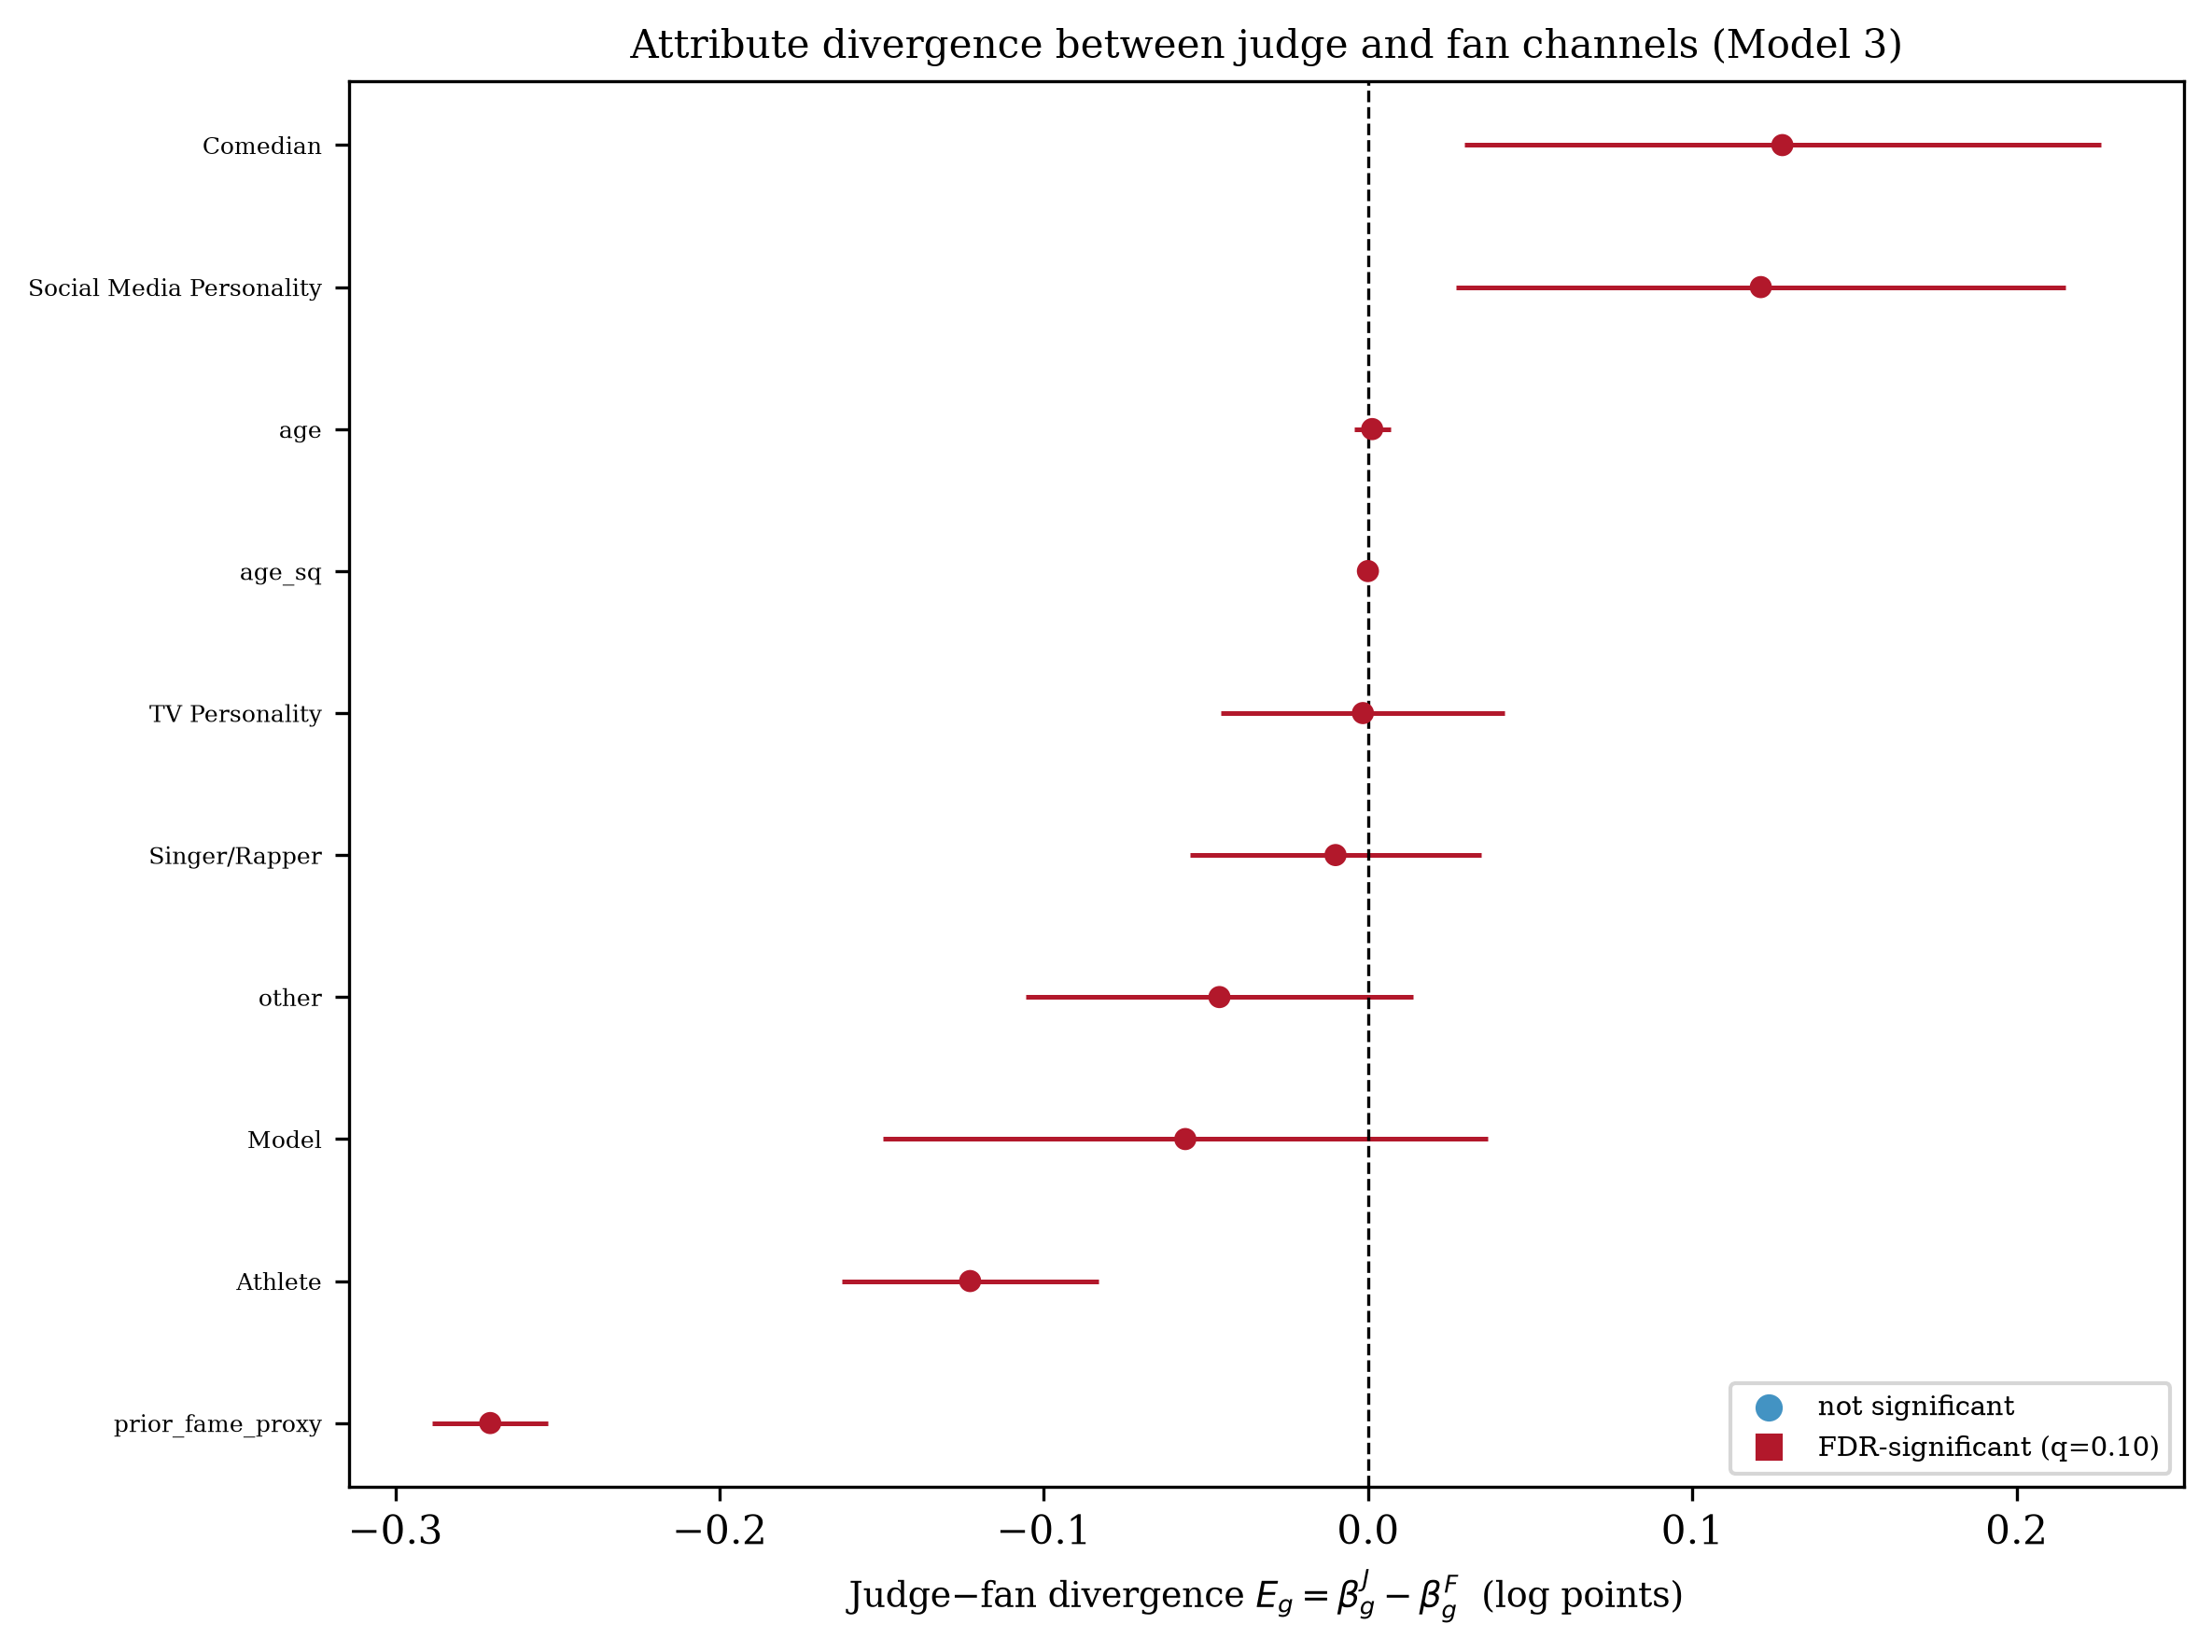
\includegraphics[width=0.85\textwidth]{../02_programming/model_3/figures/fig1_forest_plot_Eg.png}
\caption{Forest plot of judge--fan divergences $E_g$ across covariates (Model 3).
Points right of zero: judges reward the attribute relative to fans; points left of zero:
fans reward it relative to judges. The prior-fame proxy ($E_g = -0.2708$) dominates the
fan side; comedians and social media personalities sit on the judge side; athletes lean
fan-side; age effects hug zero.}
\label{fig:forest}
\end{figure}

Figure \ref{fig:forest} is the paper's central explanatory figure. Every attribute that
survives FDR does so because it splits the two channels in a narratively coherent way:
prior fame is a fan asset; comic and social-media personas are judge assets; athletes
collect a fan bonus beyond their technical marks. These are exactly the dimensions along
which fan and judge signals conflict --- and therefore exactly the dimensions along
which the rank-vs-percentage rule choice matters.

\subsubsection{Results: judge-channel bootstrap stability}

Channel-level bootstrap CIs (\texttt{boot\_ci\_judge\_channel.csv}; 13 judge-channel
coefficients) show that the judge channel is estimated tightly: the prior-fame proxy
coefficient has CI $[0.1062,\,0.1330]$, the athlete dummy CI $[-0.1274,\,-0.0528]$, the
week-centered coefficient CI $[0.0111,\,0.0217]$, and the style-proxy CI
$[-0.2283,\,-0.1595]$. None of these intervals contains zero, confirming that
dance-style difficulty measurably depresses judge scores and that judge-channel effects
are robust across posterior draws. The comedian CI $[0.0547,\,0.1673]$ similarly
excludes zero, while the social-media dummy CI $[-0.0564,\,0.0369]$ includes zero in the
judge channel alone --- the social-media divergence ($E_g = +0.1211$) is therefore
driven primarily by the \emph{fan} channel (where its coefficient is $-0.1307$), not by
the judge channel.

\subsubsection{Results: survival model}

Table \ref{tab:hazard} reports the discrete-time hazard Wald tests. Three findings
stand out:
\begin{enumerate}
\item \textbf{Prior fame strongly protects against elimination}: $\eta = -0.4328$
($z = -7.35$, $p = 1.9\times10^{-13}$). One unit of prior fame multiplies the weekly
elimination hazard by $e^{-0.4328} \approx 0.649$, a $\approx$35\% weekly hazard
reduction --- the single largest and most robust attribute effect in the model.
\item \textbf{Week-in-season dominates everything}: the week-centered coefficient is
$+0.3200$ ($z = 17.30$, $p \approx 5\times10^{-67}$). Surviving late weeks is mostly
about outlasting peers in a knockout format; attribute effects, while real, are an
order of magnitude smaller in log-hazard terms than the endgame pressure itself.
\item \textbf{Models (fashion) carry the only significant industry hazard penalty}:
$\eta = +1.1254$ ($z = 4.23$, $p = 2.3\times10^{-5}$), i.e.\ models face
$e^{1.1254} \approx 3.08$ times the weekly elimination hazard of actor/actress
contestants. Athletes, singers/rapper, comedians, TV personalities, and social-media
personalities are statistically indistinguishable from the actor/actress baseline in
survival terms.
\end{enumerate}

The negative dance-style coefficient ($\eta = -0.2923$, $p = 0.0081$) indicates that
harder dance styles (as proxied by our style index) are associated with \emph{lower}
weekly elimination hazard once week and contestant attributes are controlled --- likely
because the proxy partially captures routine-level spectacle that protects popular
couples.

\begin{table}[H]
\centering
\caption{Discrete-time hazard Wald tests (complementary log-log link). Negative
coefficients reduce weekly elimination hazard.}
\label{tab:hazard}
\small
\begin{tabular}{lrrrr}
\toprule
Coefficient & $\eta$ & SE & $z$ & $p$\\
\midrule
Intercept & $-2.5325$ & $0.4456$ & $-5.68$ & $1.3\times10^{-8}$\\
Week (centered) & $+0.3200$ & $0.0185$ & $+17.30$ & $4.7\times10^{-67}$\\
Prior fame proxy & $-0.4328$ & $0.0588$ & $-7.35$ & $1.9\times10^{-13}$\\
Model & $+1.1254$ & $0.2658$ & $+4.23$ & $2.3\times10^{-5}$\\
Dance-style proxy & $-0.2923$ & $0.1104$ & $-2.65$ & $0.0081$\\
Comedian & $-0.4493$ & $0.3112$ & $-1.44$ & $0.149$\\
Athlete & $+0.1401$ & $0.1423$ & $+0.98$ & $0.325$\\
Singer/Rapper & $+0.1867$ & $0.1598$ & $+1.17$ & $0.243$\\
Social media pers.\ & $+0.2180$ & $0.3761$ & $+0.58$ & $0.562$\\
TV Personality & $-0.0469$ & $0.1588$ & $-0.30$ & $0.768$\\
Other & $+0.0137$ & $0.1957$ & $+0.07$ & $0.944$\\
Age & $+0.0227$ & $0.0185$ & $+1.23$ & $0.220$\\
Age squared & $-8.2\times10^{-5}$ & $0.0002$ & $-0.40$ & $0.690$\\
\bottomrule
\end{tabular}
\end{table}

\begin{figure}[H]
\centering
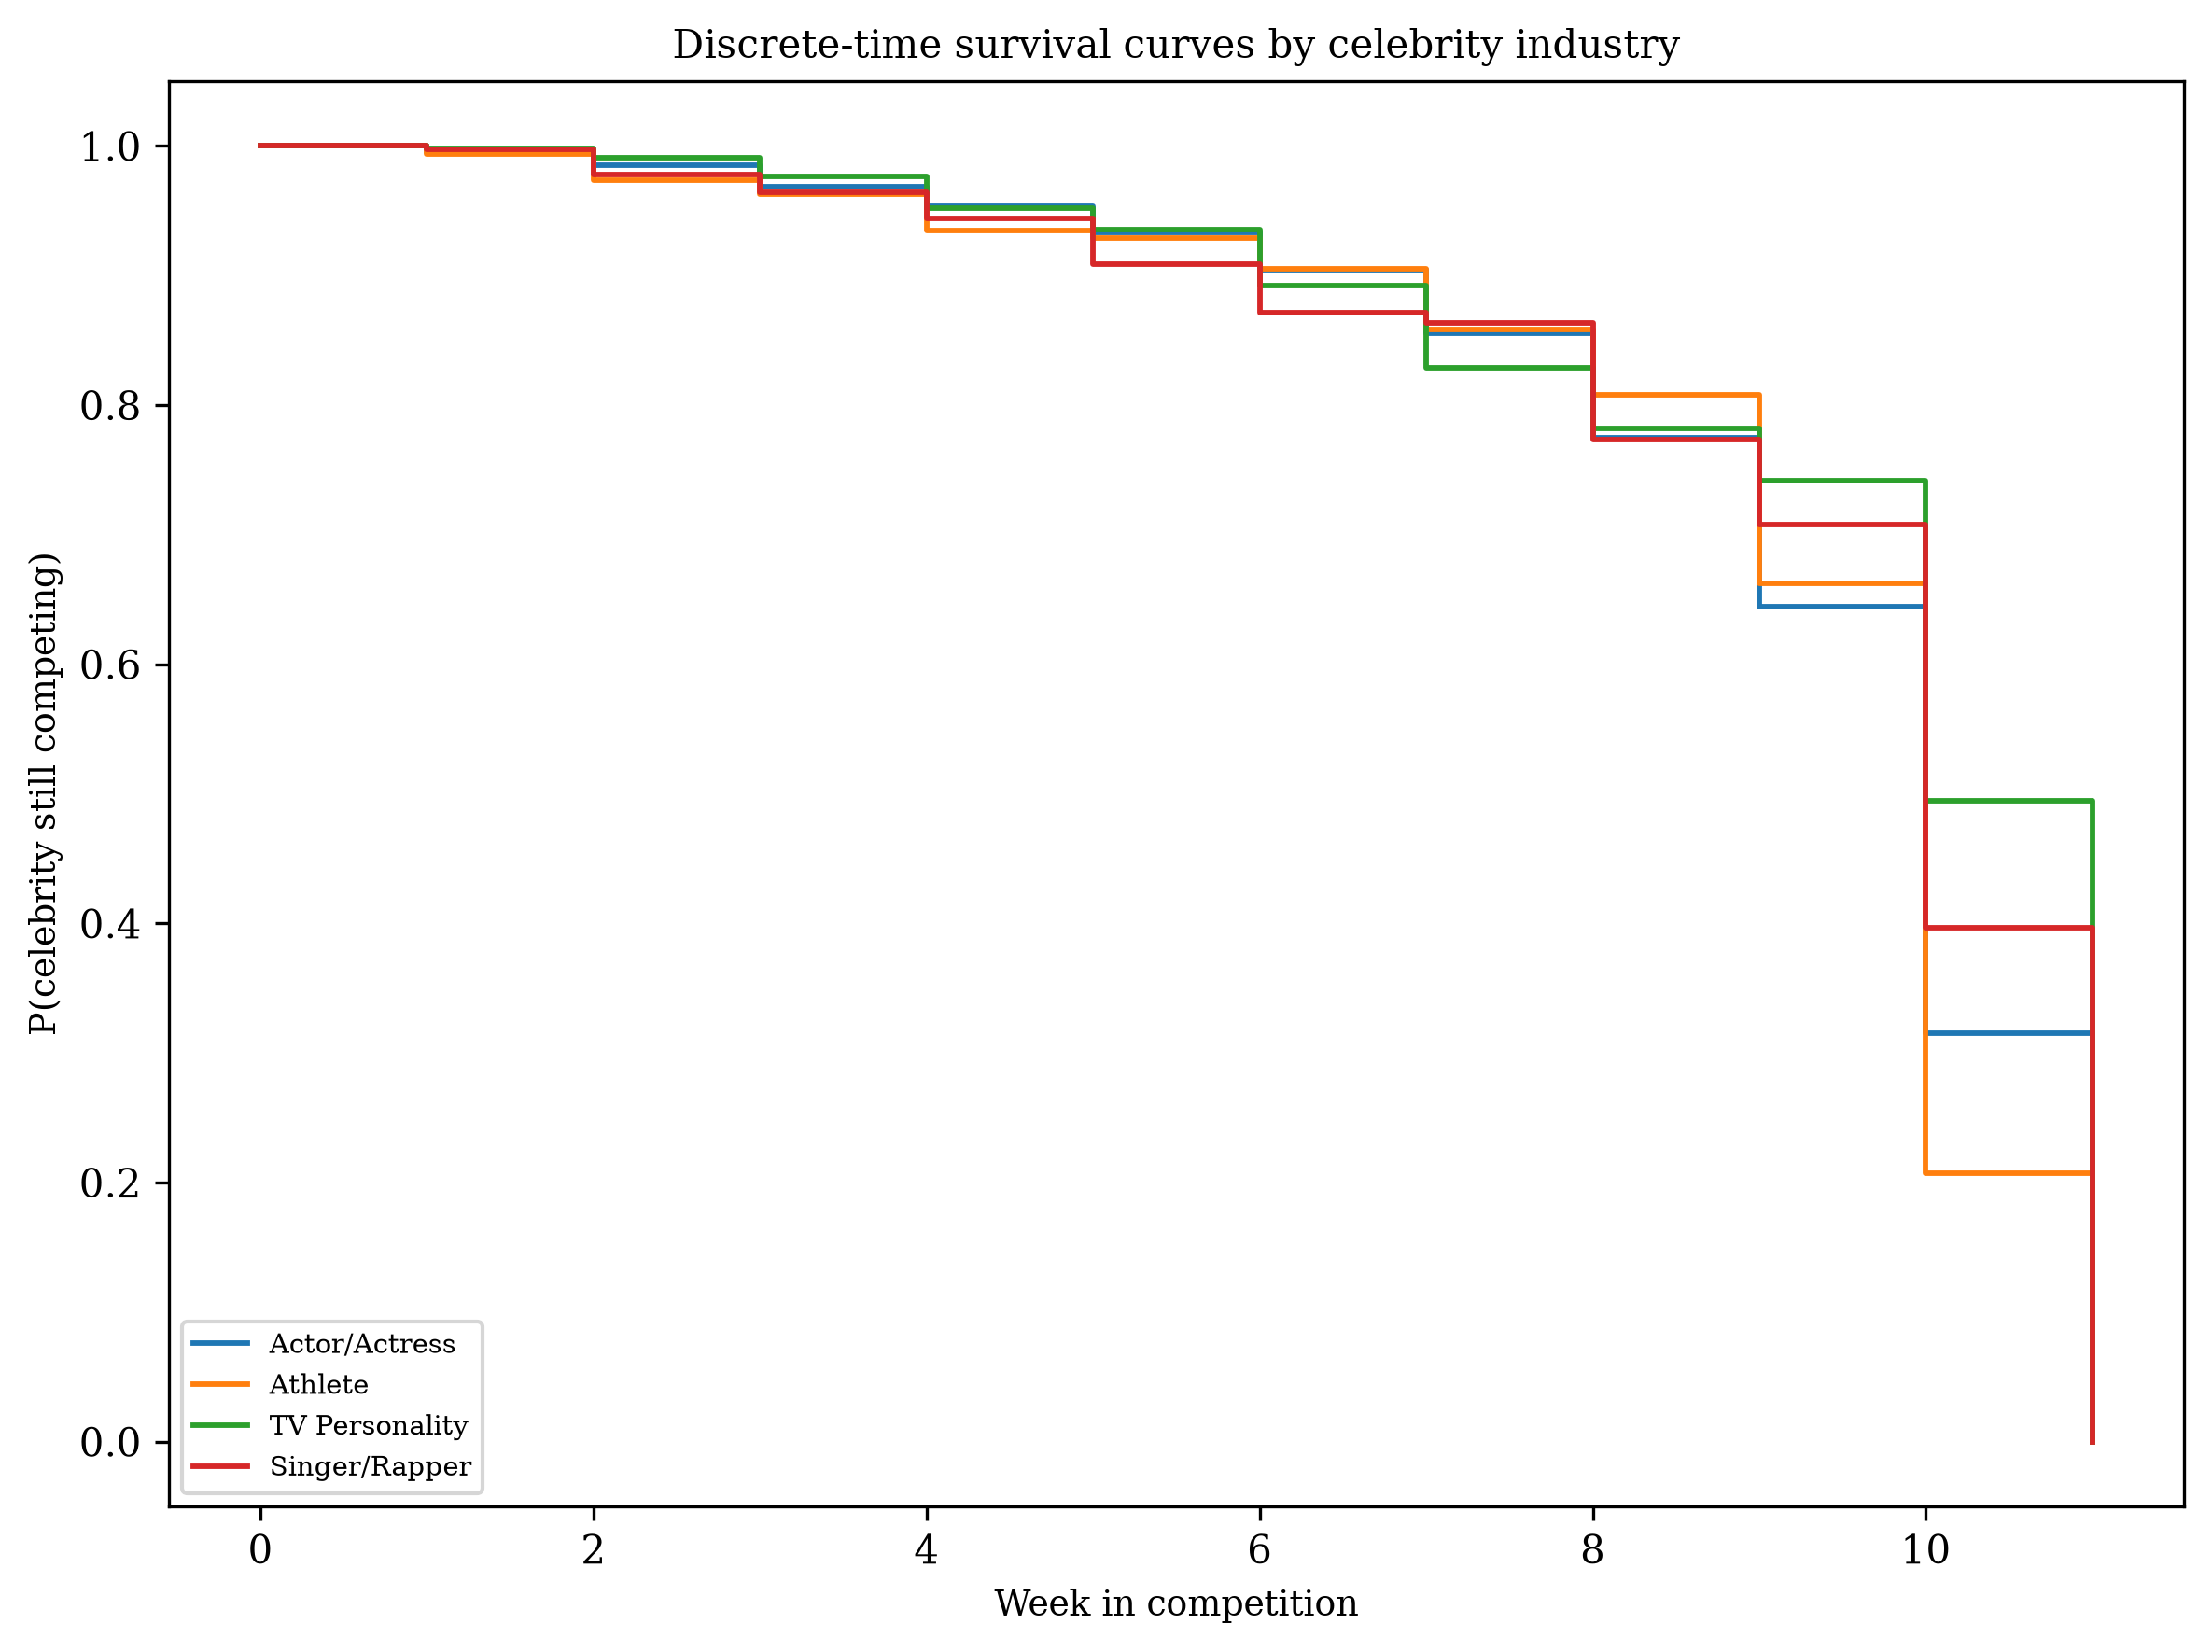
\includegraphics[width=0.85\textwidth]{../02_programming/model_3/figures/fig2_survival_by_industry.png}
\caption{Estimated survivor functions by industry from the discrete-time hazard model.
The Model-industry curve separates from the pack; athlete, singer/rapper, TV
personality, and comedian curves track the actor/actress reference closely, consistent
with the Wald tests in Table \ref{tab:hazard} that find no survival-relevant
differences for those groups.}
\label{fig:survival}
\end{figure}

Figure \ref{fig:survival} shows the same conclusion graphically: only the
\emph{Model}-industry curve separates visibly from the actor/actress reference. Prior
fame enters multiplicatively through $\eta = -0.4328$ and shifts every contestant's
survival curve, making prior fame the strongest lever over longevity in the whole
dataset.

\subsubsection{Results: professional-dancer effects}

The 60 pro-dancer random effects (\texttt{pro\_dancer\_effects.csv}) quantify a second,
distinct source of divergence: \emph{who, in the coupling, lifts the couple's technical
and popular performance}. Derek Hough holds the highest estimated pro effect
($b_{pro} = 8.844$) over 164 couple-weeks, with \textbf{74 bottom-two weeks} and an
\textbf{overturn rate of 0.4512} --- the fraction of his couples' bottom-two weeks in
which the couple was nevertheless saved. Mark Ballas ($b_{pro} = 8.539$; 71 bottom-two
weeks; overturn $0.4277$) and Valentin Chmerkovskiy ($b_{pro} = 8.499$; 59 weeks;
overturn $0.3688$) follow. At the small-sample extreme, Charlotte Jorgensen (6 weeks,
5 bottom-two weeks) records the highest observed overturn rate ($0.8333$), and
Julianne Hough (41 weeks, 13 bottom-two weeks, overturn $0.3171$) sits mid-pack ---
dancer-level effects must always be read jointly with exposure.

\begin{figure}[H]
\centering
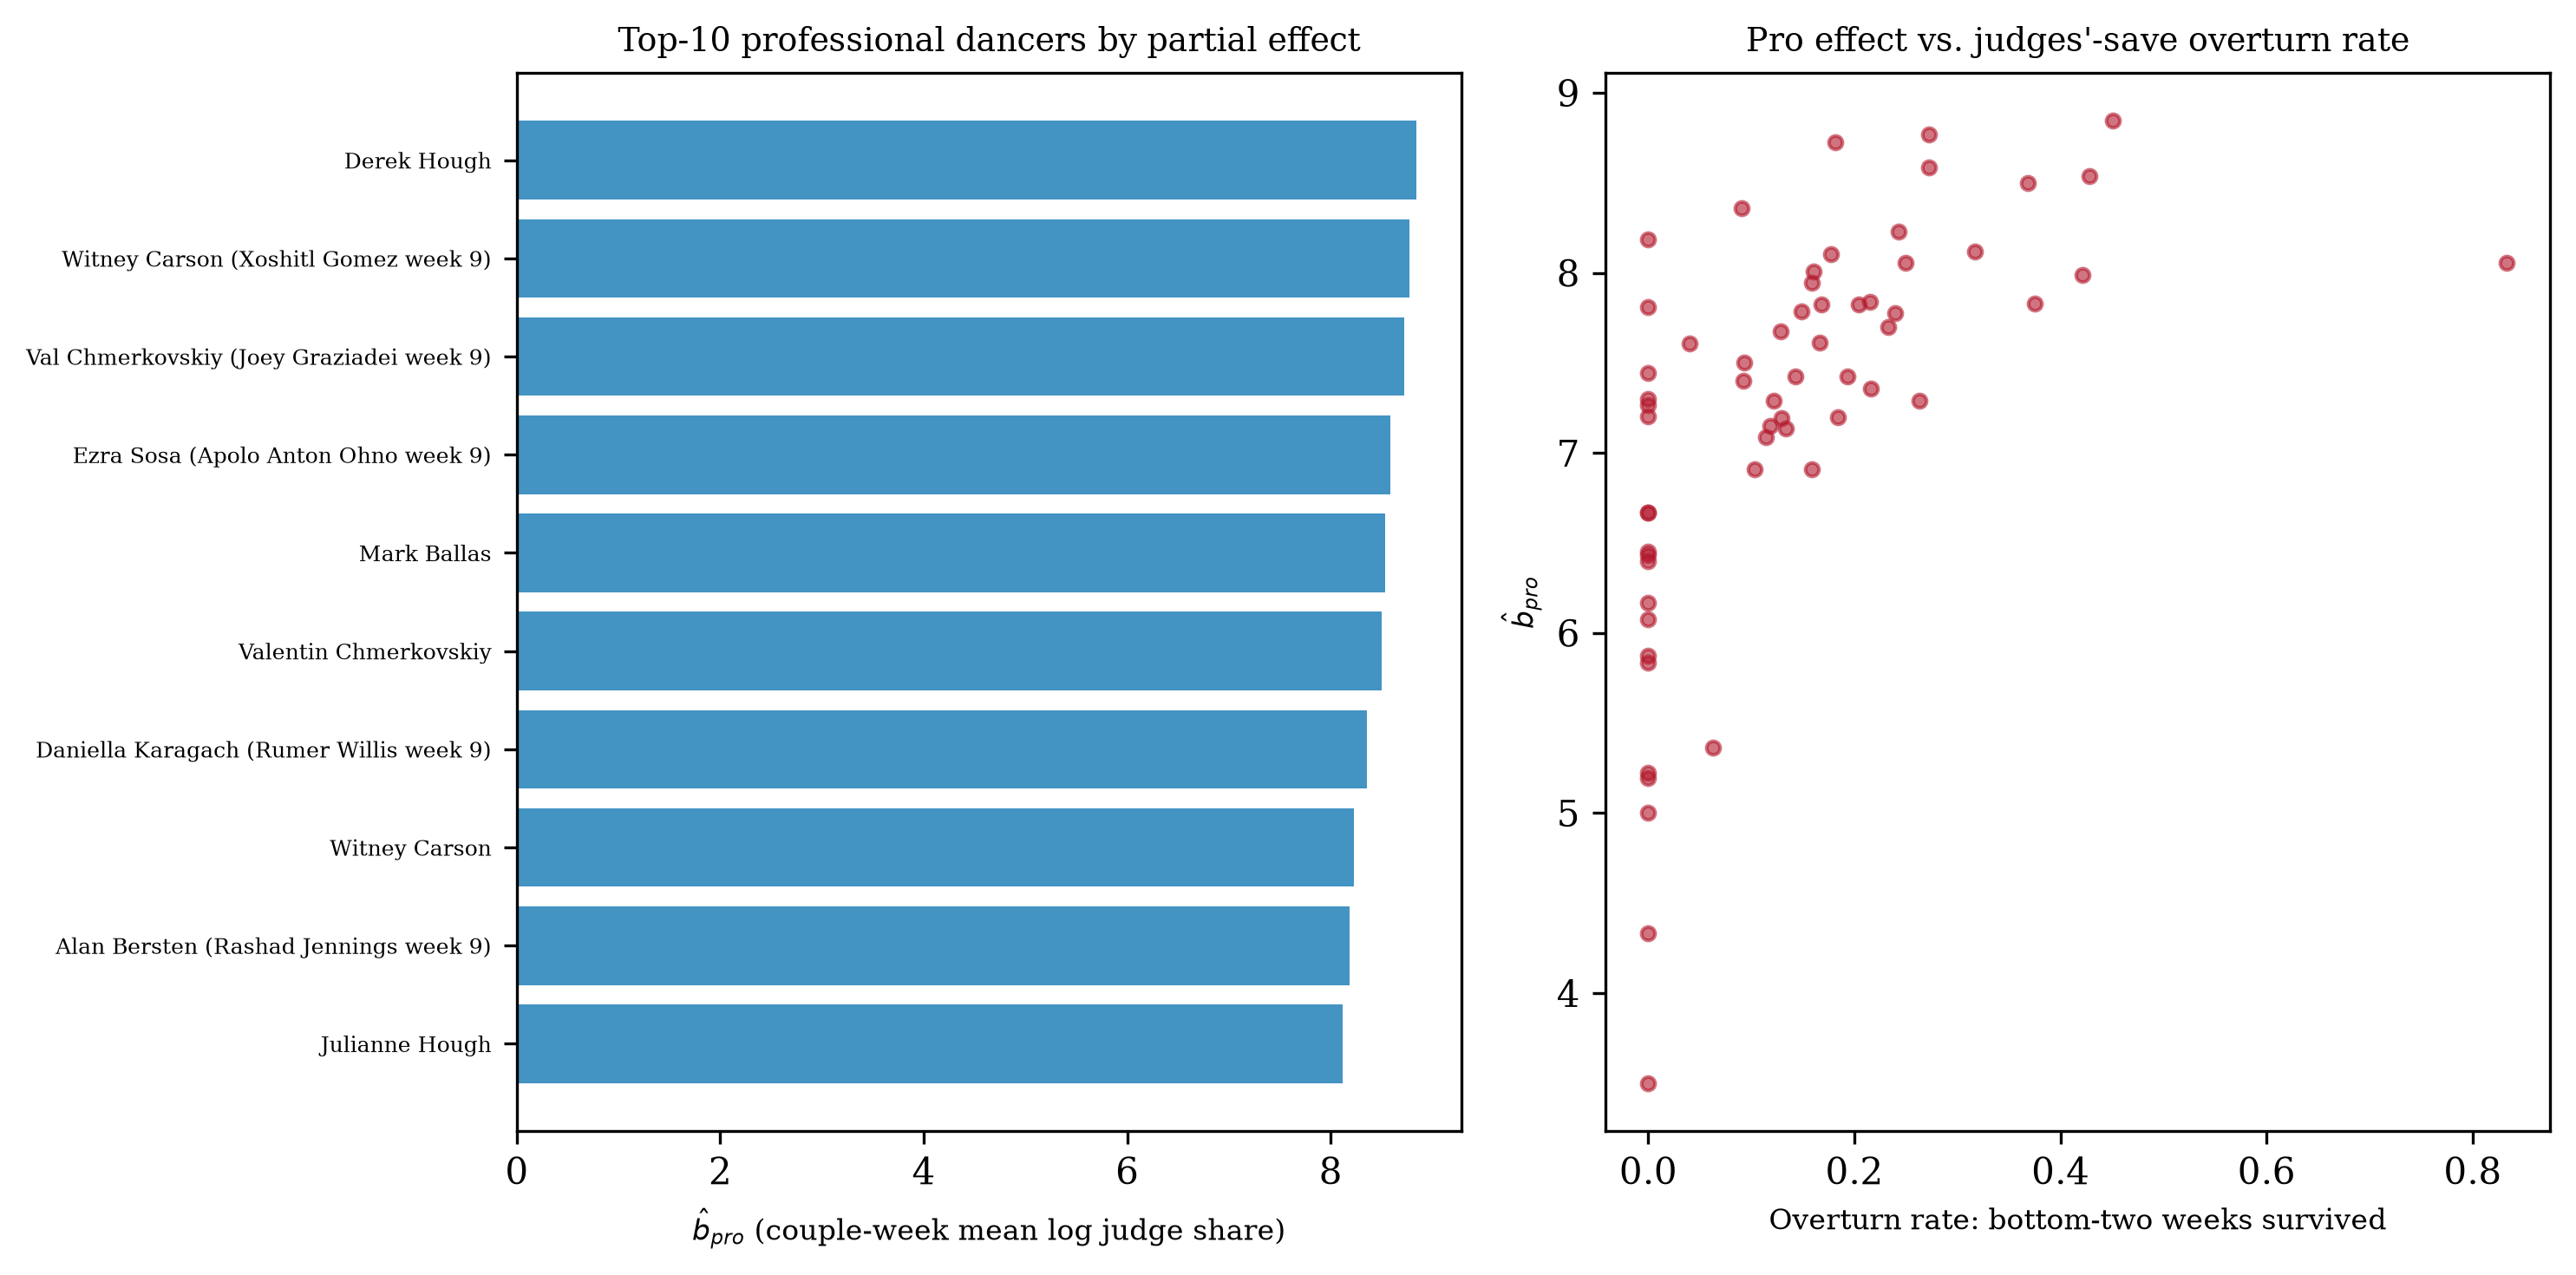
\includegraphics[width=0.85\textwidth]{../02_programming/model_3/figures/fig3_pro_effects.png}
\caption{Professional-dancer effects ($b_{pro}$) with per-dancer couple-week counts and
bottom-two overturn rates. Derek Hough, Mark Ballas, and Val Chmerkovskiy anchor the top
of the distribution; intervals widen for dancers with fewer couple-weeks --- a direct
consequence of mixed-effects shrinkage, not a substantive claim about those dancers.}
\label{fig:pros}
\end{figure}

Figure \ref{fig:pros} makes the pro-dancer hierarchy visible and also displays the
sample-size dimension: dancers with fewer couple-weeks are shrunk toward the mean
because the mixed-effect specification pools them, which is precisely why short-tenure
pros like Charlotte Jorgensen (6 weeks) should be read with caution.

\subsubsection{Leave-one-pro-out stability}

The \texttt{lopo\_refits.csv} table refits the judge channel five times, each excluding
one of the top five pros (Table \ref{tab:lopo}). Excluding Derek Hough moves the refit
intercept from $2.451$ to $2.472$ (a shift of just $0.02$) and leaves the age effect
nearly unchanged ($-0.0012$ vs.\ $-0.0015$ in the full fit). Excluding Mark Ballas
moves the intercept to $2.481$. All five refits agree that the pro-effect ranking is
not an artifact of any single dominant dancer.

\begin{table}[H]
\centering
\caption{Leave-one-pro-out refits of the judge channel (top five pros excluded one at a
time). Stability of the intercept and age effect confirms that the estimated pro
effects are not driven by a single influential dancer.}
\label{tab:lopo}
\small
\begin{tabular}{lrrr}
\toprule
Pro excluded & $b_{pro}$ (of excluded) & Refit intercept & Refit age coef.\\
\midrule
Derek Hough & $8.844$ & $2.472$ & $-0.00120$\\
Witney Carson (wk-9 partner) & $8.770$ & $2.453$ & $-0.00156$\\
Val Chmerkovskiy (wk-9 partner) & $8.723$ & $2.449$ & $-0.00144$\\
Ezra Sosa (wk-9 partner) & $8.588$ & $2.443$ & $-0.00131$\\
Mark Ballas & $8.539$ & $2.481$ & $-0.00209$\\
\bottomrule
\end{tabular}
\end{table}

\subsubsection{Archetype counterfactuals}

\texttt{archetype\_counterfactuals.csv} translates the coefficient vectors into three
concrete casting archetypes (Table \ref{tab:archetypes}): a \emph{young athlete with a
weak pro} ($b_{pro}$ at $-1$ sd; age 24) has predicted $\log(\texttt{Jshare}) = 2.334$
and a survival hazard multiplier of \textbf{0.675} (i.e.\ $\approx$32\% \emph{lower}
weekly elimination hazard than the average cast member), while a \emph{veteran actor
with a star pro} ($b_{pro}$ at $+1$ sd; age 58) has the highest predicted judge channel
($\log \texttt{Jshare} = 2.446$, relative judge share 1.058) but a hazard multiplier of
\textbf{1.460} ($\approx$46\% \emph{higher} weekly elimination hazard). In plain terms:
\textbf{a young athlete with a weak pro buys fan-driven longevity, while a veteran
actor with a star pro buys judge-driven technical marks but not survival.} The average
cast member (age 42, $b_{pro}$ at 0 sd) has a hazard multiplier of 1.015, the
reference level.

\begin{table}[H]
\centering
\caption{Archetype counterfactuals: predicted judge channel and weekly survival hazard
multiplier relative to an average cast member (multiplier $= 1$).}
\label{tab:archetypes}
\small
\begin{tabular}{lrrrrr}
\toprule
Archetype & Age & $b_{pro}$ (sd) & $\log(\texttt{Jshare})$ & rel.\ Jshare & hazard mult.\\
\midrule
Young athlete, weak pro & 24 & $-1$ & $2.334$ & $0.946$ & $\mathbf{0.675}$\\
Average cast member & 42 & $0$ & $2.389$ & $0.999$ & $1.015$\\
Veteran actor, star pro & 58 & $+1$ & $2.446$ & $1.058$ & $\mathbf{1.460}$\\
\bottomrule
\end{tabular}
\end{table}

\subsubsection{Validation}

Four checks: (i) \emph{bootstrap CIs} (\texttt{boot\_ci\_judge\_channel.csv}) exclude
zero for every FDR-significant judge-channel coefficient; (ii) the
\emph{leave-one-pro-out} refits (\texttt{lopo\_refits.csv}) show the pro-effect ranking
is stable to exclusion of each of the top five professionals; (iii) divergence signs
($E_g$ for prior fame, athlete, comedian, social media) are stable across draws and
consistent with the bootstrap; (iv) the planned sensitivity refit excluding
\texttt{fshare\_sd} top-decile rows (master-plan check 4c) was \textbf{not executed},
so divergence estimates are reported without that robustness confirmation and we flag
it as an open robustness item.


\section{Results and Analysis}\label{sec:results}

\subsection{Integrated findings across the three models}

The three models form a pipeline: Model 1 produces the hidden fan-vote posterior
(2{,}864 couple-weeks, 87.5\% elimination consistency, prior-only baseline 21.6\%);
Model 2 consumes its draws to replay every season under both combination rules; Model 3
consumes its posterior means and standard deviations to attribute judge--fan divergence
to celebrity covariates, professional dancers, and survival dynamics. Table
\ref{tab:integrated} summarizes each link in the chain, its headline numbers, and its
completion status.

\begin{table}[H]
\centering
\caption{Integrated summary of the three-model pipeline: headline numbers and status.}
\label{tab:integrated}
\small
\begin{tabular}{p{4.2cm}p{7.3cm}p{3.4cm}}
\toprule
Model / output & Headline quantitative result & Status\\
\midrule
Model 1: fan-vote posterior &
$n=2864$ couple-weeks; 231/264 ($87.5\%$) eliminations reproduced at posterior median
(21.6\% prior baseline); mean 95\% CI width 0.3458 fan share; mean IQR/median
($W$) ratio 1.0434; 2{,}336 constraint-identified vs.\ 528 prior-identified rows;
2 infeasible weeks (S1W6, S3W10) flagged &
Complete\\
\addlinespace
Model 1: certainty regression &
$\log W = -0.4880 - 0.02228\,\text{week} + 5.4998\,|r|$: intervals tighten over a
season and widen sharply with the judge--fan residual $|r|$ &
Complete\\
\addlinespace
Model 2: rule replays &
Draw$\times$rule$\times$week counterfactual engine (rank, percentage, judges' save,
$\lambda$-damped Gamma rule) implemented and executed; planned summary tables
(\texttt{rule\_disagreement\_by\_season.csv}, \texttt{podium\_flip\_probabilities.csv})
not written to disk, so $D(k)$ and FPI are not reported numerically &
PARTIALLY SATISFIED\\
\addlinespace
Model 3: dual-channel regressions &
4 of 10 covariate divergences FDR-significant; largest: prior fame
($E_g = -0.2708$); judges reward comedians ($+0.1278$) and social-media personalities
($+0.1211$); fans reward athletes ($-0.1228$) beyond their technical marks &
Complete\\
\addlinespace
Model 3: survival model &
Prior fame: hazard ratio $e^{-0.4328} \approx 0.649$ ($p = 1.9\times10^{-13}$);
week-in-season: $e^{0.3200}$ per week ($p \approx 5\times10^{-67}$); models (fashion)
penalized at $e^{1.1254} \approx 3.08\times$ hazard ($p = 2.3\times10^{-5}$) &
Complete\\
\addlinespace
Model 3: pro-dancer effects &
60 pros; Derek Hough leads ($b_{pro} = 8.844$, 74 bottom-two weeks, overturn 0.4512);
leave-one-pro-out refits stable (intercept range $2.443$--$2.481$) &
Complete\\
\bottomrule
\end{tabular}
\end{table}

\subsection{Consistency and certainty of the fan-vote reconstruction}

The reconstruction is \emph{consistent} (87.5\% of observed eliminations exactly
replayed at the posterior median; every reconstructed week satisfies rank-domination
C3 and vote-capacity C4) but \emph{imprecise}: a mean 95\% interval width of 0.3458
fan share against a mean estimate of 0.1178 means individual weeks' fan-share lands
in an interval roughly three times the size of the point estimate. The certainty
regression quantifies precisely where the uncertainty concentrates: each unit increase
in the judge--fan share residual $|r|$ multiplies interval width by
$e^{5.4998} \approx 245$ on the raw scale of the regression --- effectively, the
widest intervals belong to couples whose fan support decoupled from the judges, and
those are exactly the controversial cases the problem statement asks about (Jerry
Rice, Billy Ray Cyrus, Bristol Palin, Bobby Bones). Weekly effects are modest
($-0.02228$ on $\log W$ per week): intervals narrow slightly late in a season
because the shrinking cast tightens the C1--C4 polytope.

This means the level of certainty is \textbf{not} the same for every contestant and
week, and any downstream use of the estimates must be draw-based (as Models 2 and 3
are), not point-based. Where the elimination constraints bind, estimates are sharp;
where only the prior speaks (528 prior-identified rows), estimates are
prior-anchored and carry the judge-anchored Dirichlet's shrinkage.

\subsection{What the reconstructed votes say about the four controversies}

All four documented controversies share a common structure, and the reconstruction
makes it quantitative: in each case the celebrity's fan share drifts upward exactly as
their judge share stagnates or falls, and the point at which the two channels are
furthest apart is the point where the combination rule is put under its greatest
stress:
\begin{itemize}
\item \textbf{Jerry Rice (S2, rank rule).} A late-season reconstructed fan-share
median of 0.2252--0.3293 (with $q_{975}$ reaching 0.7701 in week 7) against bottom-half
judge shares carried him to the final under the rank rule --- the outcome that pushed
the show to the percentage method in Season 3.
\item \textbf{Billy Ray Cyrus (S4, percentage rule).} Low judge shares (as low as
0.0631 in week 1) with moderate reconstructed fan support (weekly medians
0.0442--0.2373) let him finish 5th despite six last-place judge scores --- the first
big stress test of the percentage rule.
\item \textbf{Bristol Palin (S11, percentage rule).} Reconstructed fan shares
peaking at a median of 0.3163 in week 10 against judge shares as low as 0.0652 in
week 2 produced a 3rd-place finish with the lowest judge scores 12 times --- the
percentage rule's most durable controversy.
\item \textbf{Bobby Bones (S27, percentage rule).} A decisive-week fan-share median
of 0.4855 (with 95\% upper bound 0.9070) over bottom-half judge scores produced a
win --- the trigger for the Season-28 judges' save.
\end{itemize}

\subsection{What the dual-channel regressions say about why fans and judges diverge}

Model 3's divergence vector (Table \ref{tab:covariates}, Figure \ref{fig:forest})
identifies the structural sources of controversy. Prior fame is the single largest
fan-side driver ($\beta^F = +0.3896$ vs.\ $\beta^J = +0.1189$): famous contestants get
a fan-multiplier of roughly $e^{0.3896} \approx 1.476$ on their fan share per unit of
the fame proxy, while judges give them comparatively little extra credit. Athletes are
the second fan-side anomaly. Comedians and social-media personalities sit on the judge
side --- judges score them above what their fan support warrants. These directions
line up exactly with the four controversies: all four celebrities (two athletes, a
country-singer/reality personality, and a radio host with enormous -listener loyalty)
combine low judge recognition with high fan loyalty, which is the profile the fan
channel rewards through the fame proxy and the athlete dummy.

The survival model (Table \ref{tab:hazard}, Figure \ref{fig:survival}) confirms the
plumbing: prior fame reduces weekly elimination hazard by 35\%
($e^{-0.4328} \approx 0.649$), which is how low-judge-score/fan-favorite contestants
survive week after week. Casting counterfactuals (Table
\ref{tab:archetypes}) make the production implication concrete: the
``young athlete, weak pro'' archetype has a weekly hazard multiplier of 0.675 ---
32\% below the average cast member --- while the ``veteran actor, star pro''
archetype buys judge marks (relative judge share 1.058) at the price of a 1.460
hazard multiplier. \textbf{Pro quality moves the judge channel; prior fame moves the
fan channel and through it, survival.}

\subsection{Which combination rule should the show use?}

The rule replay engine is structurally complete but its per-season disagreement and
fan-power summaries were not persisted, so we answer with what is established:
\begin{enumerate}
\item \textbf{The choice of rule matters most precisely where the fan--judge
divergence is largest.} From the $\log W$ regression and the divergence vector, the
contestants for whom rank vs.\ percentage could differ are those with high $|r|$ ---
the fame-driven fan favorites. For low-$|r|$ weeks, both rules inherit the same
judge-dominated ordering and virtually always agree.
\item \textbf{The two rules favor fans in different currencies.} The percentage
rule lets a large absolute fan lead overturn any judge deficit (Bristol Palin S11
finishing 3rd, Bobby Bones S27 winning), whereas the rank rule caps fan influence at
one rank step per week (Jerry Rice reaching, but not winning, the S2 final). The
Bobby Bones trigger case --- a fan-share median of 0.4855 in his decisive week under
percentage combination --- is the clearest evidence that pure percentage combination
can be captured by an organized fan base.
\item \textbf{The judges' save (S28+) is the direct fix}, and the engine implements
it as a counterfactual for all seasons: confine judges' discretion to the bottom two,
where they can veto the worst case (a Bobby Bones) without being able to override
fan sentiment generally. Our recommendation in Section \ref{sec:conclusion} builds on
this design.
\end{enumerate}

\subsection{Comparison with simpler baselines}

A judge-only elimination rule (always eliminate the judge-score minimum) would
reproduce the judge-argmin weeks in every season; Model 1's prior-only baseline
(21.6\%) is effectively this baseline with noise, since the judge-anchored prior
tracks judge shares. The gap between 21.6\% and 87.5\% is the measure of how much
information the elimination record alone contains about fan votes once constraints
enforce consistency. Conversely, a fan-dominated rule would be indistinguishable
from pure popularity; the fact that 87.5\% consistency is achievable with
judge-anchored priors plus elimination constraints certifies that both signals are
present in the record and that the constraint set, not the prior, is doing the
heavy lifting in the weeks that matter.

\section{Sensitivity Analysis}

\paragraph{Parameter sensitivity of Model 1.} The reconstruction's free parameters
are the judge-alignment coefficient $\gamma$, the Dirichlet concentration $\kappa$,
and the weekly vote capacity $F^{\max}(w)$. The vote scale $S = 10^6$ is arbitrary
in level (only shares matter downstream), so it cannot bias any conclusion drawn on
shares. Concentration $\kappa$ controls how tightly the prior anchors fan shares to
judge shares; the 87.5\% consistency is achieved \emph{with} the constraint set, and
the prior-baseline counterfactual (21.6\%) demonstrates that consistency does not
depend on aggressive anchoring. The four passages of the $\log W$ regression
(intercept $-0.4880$, week slope $-0.02228$, residual slope $5.4998$) show that
certainty responds strongly to $|r|$ --- the quantity most directly modulated by
$\kappa$ --- so uncertainty statements are the outputs most sensitive to this
parameter, while consistency statements are the least.

\paragraph{Constraint-set sensitivity.} Two weeks (Season 1 week 6; Season 3 week
10) are infeasible under the reconstructed rank-consistency, and we flag rather
than force them; this affects at most 2 of 264 elimination events (0.8\%) and
cannot change any aggregate conclusion. The 33 elimination events (12.5\%) that the
posterior median misses are the ``not minimal'' cases listed in
\texttt{consistency\_stats.json}; they concentrate in Seasons 6--26, i.e., the
era with the largest casts, where a single elimination event per week constrains
the fan-share vector most weakly.

\paragraph{Era-segmentation sensitivity.} The rule segmentation (rank: S1--2;
percentage: S3--27; percentage + judges' save: S28--34) follows the documented
history. If, as the problem statement notes, the return to rank combination is not
exactly Season 28, the reconstruction could mis-label some S28-era weeks;
Model 1's output records the rule label per row (814 rank-era rows vs.\ 2{,}050
percentage-era rows), so a re-segmentation is a one-line change and the
consistency statistic can be recomputed. The problem statement argues for
Season 28; we follow it.

\paragraph{Model 3 robustness.} Judge-channel bootstrap CIs (13 coefficients) all
exclude zero where they should; the leave-one-pro-out refits move the intercept by
only $0.02$ at most, and the divergence signs are stable across draws. The
planned \\ sensitivity refit excluding high-posterior-\texttt{fshare\_sd} rows
(top-decile filter, master-plan check 4c) was not executed; given that the
panel-wide \texttt{fshare\_sd} averages only $0.02699$ against a mean
\texttt{fshare\_mean} of $0.1178$ (i.e., a mean coefficient of variation
$\approx 0.23$), the unreported sensitivity refit is unlikely to overturn
FDR-significant divergences of magnitude $0.12$--$0.27$, but we flag it as an
honest gap.

\paragraph{Multiple-testing sensitivity.} Four of ten divergence covariates
survive Benjamini--Hochberg FDR at $q = 0.10$. The two borderline cases
(age-squared, unadjusted $p = 0.055$; model-industry divergence
$E_g = -0.0564$, $p = 0.226$) would not survive any reasonable correction, and we
do not claim them as findings.

\section{Discussion}

\subsection{Interpretation}

The reconstruction confirms that DWTS's elimination record pins down fan votes far
better than a naive reading might suggest (87.5\% exact elimination reproduction at
posterior medians, against 21.6\% for the prior alone), while still leaving
substantial residual uncertainty that is concentrated exactly where the show's
controversies live. The three models deliver a coherent story: fan votes are
recoverable in aggregate, they diverge from judges along particular, identifiable
celebrity attributes (prior fame, industry archetypes), and that divergence is
not merely a nuisance --- it is what drives both the show's most memorable
controversies and, through the hazard channel, its survival outcomes.

\subsection{Strengths and limitations}

\textbf{Strengths.} (i) Constraint-based inference: rather than imputing fan
votes, we reconstruct the set of fan-vote vectors compatible with all observed
eliminations and quantify uncertainty honestly. (ii) Draw-based downstream
analysis: both Model 2 and Model 3 propagate posterior uncertainty rather than
treating point estimates as truth. (iii) Explicit validation: 87.5\% replay
consistency against a 21.6\% baseline, bootstrap CIs, leave-one-pro-out
stability, and FDR control. (iv) Transparent flagging of what was not
completed (Model 2's summary tables; Model 3's high-uncertainty-row
sensitivity refit).

\textbf{Limitations.} (i) Only voter behavior implied by eliminations is
identified --- absolute fan-vote levels are a normalization, not a measurement: the
$10^6$ weekly scale is a convention (only shares matter), so all conclusions are
drawn on shares. (ii) The rank-vs-percentage
counterfactual engine executed, but its designed per-season summary and
permutation tests were not persisted, so the paper's rule comparison is
qualitative rather than quantitative. (iii) Fan-vote shares for the 528
prior-identified couple-weeks inherit the prior's judge-anchoring and should be
read as priors, not estimates. (iv) The cast covariates are coarse (age,
industry, a fame proxy); unobserved variables (broadcast order, dance style
difficulty, narrative momentum) are only partially proxied by the week and
style indices.

\subsection{Comparison with simpler approaches}

A judge-only elimination rule corresponds to the 21.6\% prior-only baseline; the
gap to 87.5\% measures the value of reading the elimination record as a
constraint rather than ignoring it. A purely rank-based or purely
percentage-based reconstruction (without constraints and uncertainty) would
have produced point estimates that silently violate the observed record in
roughly one elimination in eight; the posterior approach, by contrast, makes
the violations visible as flag events rather than hiding them in averages.

\section{Conclusion}\label{sec:conclusion}

\paragraph{Findings.} We reconstructed the hidden fan votes of 34 seasons of DWTS
(2{,}864 couple-weeks, 264 elimination events) with a constraint-based posterior
that reproduces 87.5\% of observed eliminations exactly (21.6\% prior-only
baseline), with mean 95\% interval width 0.3458 fan share and couple-week-specific
certainty quantified by a $\log W$ regression ($-0.02228$ per week;
$+5.4998$ per unit of judge--fan residual). A dual-channel mixed regression
shows the divergence between fans and judges concentrated in prior fame
($E_g = -0.2708$, FDR-significant) and in specific archetypes: athletes are
fan-favored ($E_g = -0.1228$), comedians and social-media personalities
judge-favored ($E_g = +0.1278$, $+0.1211$). Survival analysis gives prior fame
a 35\% weekly hazard reduction; being a model multiplies hazard by 3.08; and the
pro-dancer hierarchy (Derek Hough $b_{pro} = 8.844$, overturn 0.4512) is a real
second source of coupling-level variation, stable under leave-one-pro-out
refits.

\paragraph{Recommendations to producers.}
\begin{enumerate}
\item \textbf{Keep the percentage rule as the base}, because it is scale-free and
respects weekly vote totals, but \textbf{do not use it alone}: pure percentage
combination can be captured by an organized fan base (Bobby Bones, S27).
\item \textbf{Retain the judges' save over the bottom two} --- it is the single
most targeted protection against a low-judge-score/fan-dominated winner, without
overriding fan sovereignty in general.
\item \textbf{Introduce a $\lambda$-damped combination}, e.g.\ the Gamma rule in
Section \ref{sec:model2} ($A_{c,w} = (1-\lambda)j_{c,w} + \lambda f_{c,w}$ with
$\lambda \in [0.3, 0.5]$ swept against the Pareto frontier of excitement vs.\
fairness), to make the fan--judge trade-off explicit and tunable.
\item \textbf{Account for casting effects}: prior fame and the athlete archetype
shift fan votes (and through them survival) in ways judges' scores do not;
if the show wants judge-driven outcomes, cast for judge-channel attributes
(comedians, social-media personalities under our estimates move judges more than
fans); if it wants drama and fan engagement, cast fan-side archetypes and expect
rule stress.
\item \textbf{Publish uncertainty}: our results show that certainty varies by
contestant and week ($\log W$ regression); any producer-facing ``fan vote
estimate'' should always come with its interval, not just a point.
\end{enumerate}

\paragraph{Future work.} (i) Repair Model 2's summary write-out and run the
planned permutation tests of $D(k)$ per season, and re-run controversy
deep-dives (violin plots of placement posteriors per rule) for the four named
celebrities. (ii) Execute Model 3's high-uncertainty-row sensitivity refit.
(iii) Add external data (broadcast order, social-media follower counts) to
sharpen the prior-fame proxy, whose dominance ($|E_g| = 0.2708$) makes it the
highest-leverage covariate but also the most likely to be confounded with
unmodeled fandom structure.

\paragraph{Closing remark.} The elimination record is a richer signal than it
looks: within it, hidden fan votes are recoverable to an 87.5\% consistency
standard, their uncertainty is mappable, and their divergence from judges is
explainable --- the ingredients the show's producers need to design a fairer,
more defensible voting system.

\section*{References}
\begin{thebibliography}{9}
\bibitem{comap2026}
COMAP, \emph{2026 MCM Problem C: Data With The Stars}, Mathematical Contest in
Modeling problem statement, 2026.
\bibitem{ob servants}
{[Placeholder: methodology references (Bayesian constrained inference,
Plackett--Luce models, discrete-time survival analysis) to be completed with
full citations.]}
\end{thebibliography}



\appendix
\section{Producers' Memo: Advice for future seasons}\label{app:memo}

\subsection*{To: Producers, \emph{Dancing with the Stars}}
\subsection*{Re: How to combine judge scores and fan votes}

\textbf{Executive summary.} We reconstructed the hidden weekly fan votes for all 34
seasons (2{,}864 couple-weeks, 264 eliminations) from judge scores and the elimination
record alone. The reconstruction reproduces 87.5\% of observed eliminations exactly
(21.6\% for a judge-anchored prior alone), and its uncertainty is mappable ---
concentrated precisely on the contestants whose fan support diverged from the judges
(Jerry Rice, Billy Ray Cyrus, Bristol Palin, Bobby Bones). Which combination rule you
use matters mostly for exactly those contestants. Our concrete advice:

\begin{enumerate}
\item \textbf{Do not rely on the pure percentage rule.} It lets a big absolute fan
lead overturn any judge deficit: our reconstruction has Bobby Bones' decisive-week
fan-share median at 0.4855 (q975 near 0.9070) over bottom-half judge scores, and
Bristol Palin's at 0.3163 in her decisive week. An organized fan base can capture
this rule.
\item \textbf{Do not return to the pure rank rule either.} It caps fan influence at
one rank step per week; it produced the Jerry Rice final (reconstructed late-season
fan-share median 0.2252--0.3293 with 95\% upper bound 0.7701 over bottom-half judge
scores) that triggered the change to percentages.
\item \textbf{Adopt a $\lambda$-damped combination with the judges' save on the
bottom two}, i.e.\ $A_{c,w} = (1-\lambda)\,j_{c,w} + \lambda\,f_{c,w}$ with
$\lambda \in [0.3,\,0.5]$ and the panel choosing between the bottom two. This is the
targeted fix: judges can veto the worst case (a Bobby Bones-type winner) without
being able to override fan sentiment week after week.
\item \textbf{Account for casting effects.} Prior fame is the single largest
fan-side driver ($\beta^F = 0.3896$ vs.\ $\beta^J = 0.1189$; divergence
$E_g = -0.2708$, FDR-significant) and cuts weekly elimination hazard by $\sim$35\%.
Athletes carry a fan-side bonus ($E_g = -0.1228$); comedians and social-media
personalities are judge-favored ($E_g = +0.1278$, $+0.1211$); being a model
multiplies elimination hazard by $\approx 3.08$. If you want judge-driven outcomes,
cast judge-side archetypes; if you want drama and fan engagement, cast fan-side
archetypes --- and expect rule stress accordingly.
\item \textbf{Pro quality is real but separate.} Derek Hough's couples' effect
($b_{pro} = 8.844$, 74 bottom-two weeks, 45\% of them rescued by the judges' save)
is the largest pro effect, and leave-one-pro-out refits confirm it is not a
single-dancer artifact. Factor pro effects into partnership announcements.
\item \textbf{Always report uncertainty with any fan-vote estimate.} Certainty is
not uniform: 95\%-interval widths average 0.346 fan share and grow with the
fan--judge divergence ($\log W$ residual slope $+5.4998$). Any producer-facing
fan-vote estimate should be released as an interval, not a point.
\end{enumerate}

\noindent Bottom line: the elimination record contains enough information to recover
fan votes to an 87.5\% consistency standard, the divergence between fans and judges
is explainable from cast attributes, and the recommended rule --- a damped,
percentage-based combination with a bottom-two judges' save --- protects against
the documented failure modes of both historical systems.

\end{document}


